% PAPRIKA v2 pitch deck (spec revision v2.5) - first draft (7 slides, 5 minutes).
% Same preamble, colours and layout as the sibling ORIGO draft (crypto/slides/draft/deck-draft.tex),
% so the two decks can be compared on equal terms.
% Build: pdflatex deck-draft.tex (twice). Coordinates are millimetres from the top-left corner
% of a 160 x 90 mm page.
% Every number carries a comment with the file it comes from. NOT YET CLAIM-AUDITED.
\documentclass[aspectratio=169,10pt]{beamer}
\usepackage[T1]{fontenc}
\usepackage{helvet}
\usepackage{tikz}
\usepackage{graphicx}
\usetikzlibrary{calc,arrows.meta}
\definecolor{ink}{HTML}{14123A}
\definecolor{paper}{HTML}{F8F6F1}
\definecolor{lilac}{HTML}{E4DCFB}
\definecolor{lemon}{HTML}{FFF8B8}
\definecolor{mint}{HTML}{C9F2D6}
\definecolor{rose}{HTML}{FFD9D2}
\definecolor{peach}{HTML}{FFE3C7}
\definecolor{sky}{HTML}{DCE6FF}
\definecolor{accent}{HTML}{3B45B5}
\setbeamercolor{background canvas}{bg=paper}
\setbeamercolor{normal text}{fg=ink}
\setbeamertemplate{navigation symbols}{}
\renewcommand{\familydefault}{\sfdefault}
\setbeamertemplate{footline}{}
\hyphenpenalty=10000 \exhyphenpenalty=10000
% --- layout helpers: everything is placed at absolute positions -------------------------------
\newcommand{\at}[2]{($(current page.north west)+(#1mm,-#2mm)$)}
% \card{x}{y}{width}{height}{fill}{content}
\newcommand{\card}[6]{%
  \fill[ink,rounded corners=2.5pt] ($(current page.north west)+(#1mm,-#2mm-0.8mm)$) rectangle ++(#3mm,-#4mm);
  \draw[ink,line width=0.8pt,rounded corners=2.5pt,fill=#5] \at{#1}{#2} rectangle ++(#3mm,-#4mm);
  \node[anchor=north west,inner sep=0pt,text width=#3mm-5mm,align=left,font=\scriptsize] at ($(current page.north west)+(#1mm+2.5mm,-#2mm-2.5mm)$) {#6};}
\newcommand{\head}[2]{%
  \node[anchor=north west,inner sep=0pt,font=\tiny\bfseries] at \at{9}{7} {\MakeUppercase{#1}};
  \node[anchor=north west,inner sep=0pt,font=\LARGE\bfseries] at \at{9}{11} {\MakeUppercase{#2}};
  \node[anchor=south west,inner sep=0pt,font=\tiny\bfseries] at \at{9}{86.5} {PAPRIKA};
  \node[anchor=south east,inner sep=0pt,font=\tiny,text=ink!70] at \at{151}{86.5} {IXH26 $\cdot$ TRACK 1 $\cdot$ \insertframenumber/\inserttotalframenumber};}
\newcommand{\num}[1]{\tikz[baseline=(n.base)]\node(n)[circle,draw=ink,line width=0.7pt,fill=white,inner sep=0.6pt,font=\tiny\bfseries,minimum size=3.4mm]{#1};}
\newcommand{\ct}[1]{{\small\bfseries #1}\\[1mm]}
\tikzset{flow/.style={-{Stealth[length=1.8mm]},line width=0.8pt,draw=ink}}
\begin{document}


% ============================================================ 1 Title
\begin{frame}[plain]
\begin{tikzpicture}[remember picture,overlay]
  \fill[mint] (current page.north west) rectangle \at{78}{90};
  \node[anchor=north west,inner sep=0pt,font=\tiny\bfseries,text width=62mm,align=left] at \at{9}{10} {IXH26 $\cdot$ TRACK 1 $\cdot$ UNIVERSAL PHOTO-ORIGIN VALIDATION PROTOCOL};
  \node[anchor=north west,inner sep=0pt,font=\fontsize{40}{42}\selectfont\bfseries] at \at{8.4}{22} {PAPRIKA};
  \node[anchor=north west,inner sep=0pt,font=\large\bfseries,text width=62mm,align=left] at \at{9}{42} {Staked device keys,\\ open challenge,\\ no owner.};
  \node[anchor=south west,inner sep=0pt,font=\tiny,text=ink!75] at \at{9}{84} {Team name $\cdot$ members};
  \node[anchor=north west,inner sep=0pt,font=\tiny\bfseries,text=ink!75] at \at{87}{14} {WHAT A RECORD PROVES};
  % Claim: spec/PROTOCOL.md section 1 (revision v2.4), shortened, not strengthened.
  \node[anchor=north west,inner sep=0pt,font=\normalsize,text width=64mm,align=left] at \at{87}{19}
    {The holder of device key $K$ \textbf{signed photo digest $H$} after block $b_0$ and before block $b_1$;\\[1.5mm]
     $K$ was registered with a \textbf{stake $S$}, forfeited when evidence against $K$ or the record is accepted;\\[1.5mm]
     and everything proven or decided about $K$ since is public, with its block.};
  \card{87}{63}{64}{12}{rose}{\textbf{Not claimed:} that $H$ came from a camera. For a self-registered key the guarantee is economic.}
\end{tikzpicture}
\end{frame}

% ============================================================ 2 Problem
\begin{frame}[plain]
\begin{tikzpicture}[remember picture,overlay]
  \head{The starting point $\cdot$ Apple Reference Image}{Close to a solution, but centralised}
  \card{9}{27}{68}{47}{white}{\ct{The brief, slide 10, quoted}
    \textbf{Single point of failure.} ``Apple maintains central revocation lists. A compromised CA invalidates millions of devices.''\\[2mm]
    \textbf{Cross-platform lock-in.} ``Non-Apple devices cannot natively verify claims without relying on Apple servers.''\\[2mm]
    \textbf{Retroactive censorship.} ``Historic photos become unverifiable if central servers shut down or alter public keys.''}
  \card{81}{27}{70}{47}{lemon}{\ct{Where we started: the original idea}
    Register a key $\cdot$ attest $\mathrm{SHA}(photo)$ for a fee into a treasury $\cdot$ ban a device when an oracle says a photo is fake.\\[1.5mm]
    \textbf{We attacked it on a local chain:}\\[0.8mm]
    $\bullet$ a 1\,ETH treasury drained in 21 self-report cycles % experiments/p01-paprika-baseline-attacks/README.md, attack 4
    \\[0.5mm]
    $\bullet$ one ban made 100 of 100 earlier records unverifiable % p01 README, attack 6 (invalidates-past)
    \\[0.5mm]
    $\bullet$ a copied transaction stole the origin; random bytes verified as ``attested'' % p01 README, attacks 3 and 2
    \\[1.5mm]
    {\color{ink!70}Paprika v2 is the hardened version, attacked the same way.}}
  \node[anchor=north west,inner sep=0pt,font=\scriptsize,text width=142mm,align=left] at \at{9}{79}
    {\textbf{Our test for each weakness:} is it \textbf{removed}, or only \textbf{moved} somewhere else?};
\end{tikzpicture}
\end{frame}

% ============================================================ 3 Protocol
\begin{frame}[plain]
\begin{tikzpicture}[remember picture,overlay]
  \head{The protocol $\cdot$ four steps, one contract}{Stake, sign, verify, challenge}
  \card{9}{27}{33.5}{33}{sky}{\num{1} \textbf{\small REGISTER}\\[1mm] A P-256 device key, its signature on the owner's address, and a \textbf{stake}.\\[1mm]
    \textbf{Level 0:} self-registered.\\ \textbf{Level 1:} also endorsed by a \textbf{bonded issuer}.}
  \card{45.2}{27}{33.5}{33}{lilac}{\num{2} \textbf{\small SIGN \& RECORD}\\[1mm] The device signs the photo digest and a \textbf{recent block hash}. Anyone relays it; the contract checks the signature.\\[1mm] {\color{ink!70}$\Rightarrow$ record $(H, K, b_0, b_1)$}}
  \card{81.4}{27}{33.5}{33}{mint}{\num{3} \textbf{\small VERIFY}\\[1mm] Anyone hashes the file and reads the chain: time window, level, flags, \textbf{stake still at risk}.\\[1mm] {\color{ink!70}$\Rightarrow$ no company server}}
  \card{117.6}{27}{33.4}{33}{rose}{\num{4} \textbf{\small CHALLENGE}\\[1mm]
    $\bullet$ proof of \textbf{key misuse}, checked by the contract\\[0.5mm] $\bullet$ committed \textbf{claim}, decided by vote\\[1mm] {\color{ink!70}$\Rightarrow$ flag $K$, slash $S$}}
  \draw[flow] \at{42.5}{43} -- \at{45.2}{43};
  \draw[flow] \at{78.7}{43} -- \at{81.4}{43};
  \draw[flow] \at{114.9}{43} -- \at{117.6}{43};
  \card{9}{66}{142}{14}{white}{\textbf{\color{accent}ON-CHAIN: ONE IMMUTABLE CONTRACT}\\[0.8mm]
    A flag stops new records and erases nothing. Slashing: half the stake to the challenger, the rest burned. % alpha = 0.5: spec/PROTOCOL.md section 8
    Measured gas: register 147\,k (level 0) / 182\,k (level 1), attest 64\,k. % experiments/p03-paprika-v2-hardened/README.md, "Gas, v2.4": 146,837 / 181,749 / 63,980
    }
\end{tikzpicture}
\end{frame}

% ============================================================ 4 What the contract does
\begin{frame}[plain]
\begin{tikzpicture}[remember picture,overlay]
  \head{Why a blockchain}{Removed, or moved?}
  \card{9}{27}{92}{14.5}{rose}{\textbf{Single point of failure} $\rightarrow$ \textbf{No owner, no admin, no upgrade path, no CA.}\\ \textbf{Removed} for the contract. \textbf{Moved:} claims to the oracle's token vote; at level 1, each issuer a verifier trusts is a trust root.}
  \card{9}{44}{92}{14.5}{peach}{\textbf{Cross-platform lock-in} $\rightarrow$ \textbf{Open admission; verifying needs chain data and SHA-256.}\\ \textbf{Removed} for vendors. Remains: one chain, a node to read it, and at level 1 the verifier's own list of issuers.}
  \card{9}{61}{92}{14.5}{lemon}{\textbf{Retroactive censorship} $\rightarrow$ \textbf{Records are never erased; flags are dated.}\\ \textbf{Narrowed, not removed:} a thief who proves misuse of a stolen key makes its whole archive distrusted. The records stay; the trust goes.}
  \card{105}{27}{46}{48.5}{white}{\ct{The contract's functions}
    \num{1}\; \texttt{register}, \texttt{registerIssuer}\\[1.1mm]
    \num{2}\; \texttt{attest} --- any relayer\\[1.1mm]
    \num{3}\; \texttt{proveKeyMisuse} --- no vote\\[1.1mm]
    \num{4}\; \texttt{requestUnbond}, \texttt{withdraw}\\[1.1mm]
    \num{5}\; \texttt{commitClaim}, \texttt{revealClaim}\\[1.1mm]
    \num{6}\; \texttt{verify} --- returns everything\\[1.4mm]
    {\color{ink!70}No treasury: ETH leaves as a returned stake, a reward or a burn.}}
  \node[anchor=north west,inner sep=0pt,font=\scriptsize,text width=142mm,align=left] at \at{9}{79}
    {Measured: \textbf{100 of 100} earlier records returned after a flag; \textbf{0} invariant violations in 5\,$\times$\,5{,}000 random steps (v2.3; v2.4 pending). % p03 README: attack 6 (100/100, "as v2.3" for v2.4); v2.3 fuzz section (5 seeds x 5,000 steps, 0 violations); v2.4 fuzz result is still a placeholder
    };
\end{tikzpicture}
\end{frame}

% ============================================================ 5 Crypto and economic idea
\begin{frame}[plain]
\begin{tikzpicture}[remember picture,overlay]
  \head{The cryptographic and economic idea}{A key that incriminates itself}
  \card{9}{24}{68}{26}{sky}{\ct{Signed on the device, checked on-chain}
    \mbox{$\sigma = \mathrm{Sig}_K(\texttt{CAPTURE} \| \ldots \| K \| H \| \mathrm{blockhash}(b_0))$}\\[1mm]
    \textbf{ECDSA P-256}, verified by the precompile at \texttt{0x100}.\\
    \textbf{Not before} $b_0$: its hash is unpredictable earlier.\\ \textbf{Not after} $b_1$: the block holding the record.
    }
  \card{81}{24}{70}{26}{lilac}{\ct{Two ways to challenge}
    \textbf{Key misuse:} $\mathrm{Sig}_K(\texttt{EXTRACTED} \| \ldots \| \mathit{challenger})$ shows $K$ left the capture pipeline.\\[0.5mm]
    \textbf{Claim:} committed, always contested, decided by vote; tested against an oracle mock only. Not a deepfake detector.}
  \card{9}{54}{68}{20}{white}{\ct{Two assurance levels}
    \textbf{Level 0:} self-registered; economic guarantee only.\\
    \textbf{Level 1:} endorsed by an issuer bonded with 1\,ETH; a misuse proof also earns a 0.1\,ETH bounty. Bounty $<(1-\alpha)S$: self-revocation loses. % spec section 8: ISSUER_MIN_BOND 1, ISSUER_BOUNTY 0.1 < 0.125
    }
  \card{81}{54}{70}{20}{mint}{\ct{Incentives}
    $S = 0.25$\,ETH, $\alpha = 50\%$, claim bond 0.11\,ETH. % spec/PROTOCOL.md section 8
    Self-report loses $(1-\alpha)S$; no treasury. Deters a forgery only if $p(1-\alpha)S > G$: about 4--40\,USD at $p$ = 1--10\% (\textbf{assumed} inputs). % spec section 8 and experiments/p06-economic-model/README.md: p and G assumed, ETH = 3,000 USD assumed
    }
  \node[anchor=north west,inner sep=0pt,font=\tiny,text width=142mm,align=left] at \at{9}{76.5}
    {\textbf{Withdrawn.} A third, objective challenge rule was tried, broken by an independent review with running exploits, and withdrawn.\\[0.6mm]
     \textbf{Prior work.} Deposit-bound keys: Kiayias and Tang (CCS 2013, 2015); Ruffing, Kate and Schr\"oder (CCS 2015). We assemble; we do not claim the primitive.};
\end{tikzpicture}
\end{frame}

% ============================================================ 6 Demo
\begin{frame}[plain]
\begin{tikzpicture}[remember picture,overlay]
  \head{Live demo}{Sign a photo, then try to cheat}
  \fill[ink,rounded corners=2.5pt] ($(current page.north west)+(9mm,-27.8mm)$) rectangle ++(84mm,-52mm);
  \draw[ink,line width=0.8pt,rounded corners=2.5pt,fill=white] \at{9}{27} rectangle ++(84mm,-52mm);
  \IfFileExists{../../impl/mock/mock-verify-ok.png}{%
    \node[anchor=center,inner sep=0pt] at \at{51}{53} {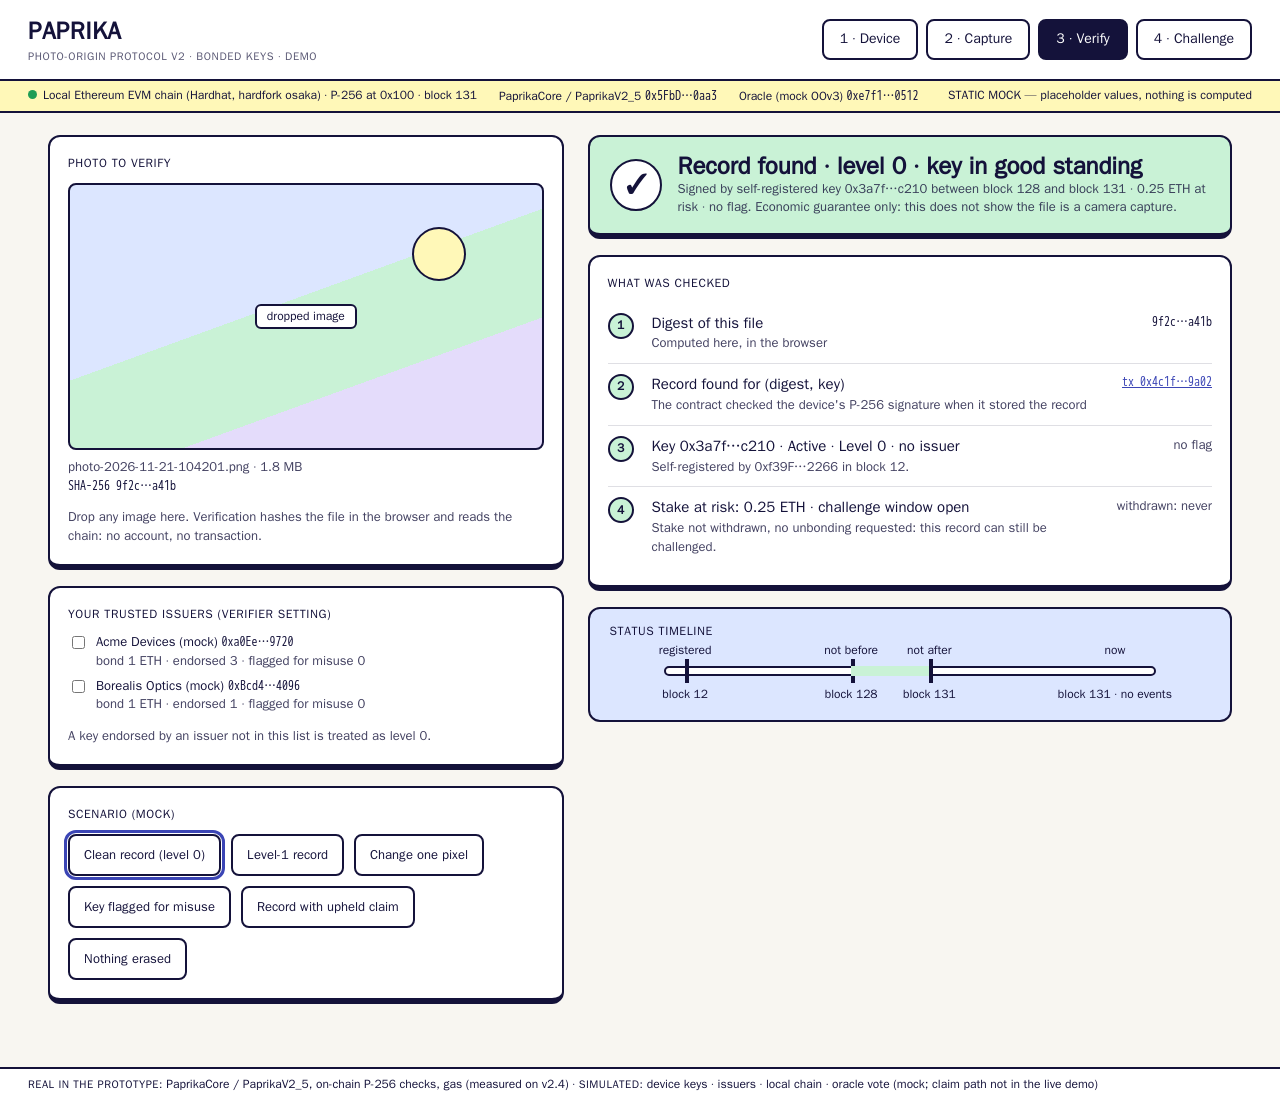
\includegraphics[width=81.6mm,height=49.6mm,keepaspectratio]{../../impl/mock/mock-verify-ok.png}};
  }{%
    \draw[ink!50,dashed,line width=0.6pt] \at{13}{31} rectangle ++(76mm,-44mm);
    \node[font=\scriptsize,text=ink!60,align=center] at \at{51}{53} {Screenshot placeholder\\ (verify page of the running prototype)};
  }
  \card{97}{27}{54}{52}{white}{\ct{The 90-second story}
    \num{1}\; Register a device key with a 0.25\,ETH stake % spec/PROTOCOL.md section 8 (MIN_STAKE)
    \\[1.4mm]
    \num{2}\; Sign a photo; a relayer records it; verify shows $[b_0, b_1]$\\[1.4mm]
    \num{3}\; Change one pixel: no record\\[1.4mm]
    \num{4}\; Extracted key: anyone proves misuse; flag, half the stake to the challenger, half burned; old records stay, marked % spec section 8, alpha = 0.5
    \\[1.4mm]
    \num{5}\; Verify again: the flag's block and reason, next to the earlier records}
  \node[anchor=north west,inner sep=0pt,font=\tiny,text=ink!70,text width=142mm] at \at{9}{81} {Static mock-up; its labels and 0.1\,ETH stake predate the current parameters. Local Ethereum EVM chain; device key in software; no public network is used.};
\end{tikzpicture}
\end{frame}

% ============================================================ 7 Limits
\begin{frame}[plain]
\begin{tikzpicture}[remember picture,overlay]
  \head{Honest limits and the road ahead}{What we do not claim}
  \card{9}{25}{80}{42}{rose}{\ct{Limits (spec, section 9)}
    $\bullet$ A level-0 record does not prove physical origin; level 1 only as far as the issuer is honest and trusted\\[0.4mm]
    $\bullet$ The stake bounds the punishment, not the damage\\[0.4mm]
    $\bullet$ Claims wait two to three days for a token vote we do not control % spec section 9, item 3
    \\[0.4mm]
    $\bullet$ An owner can self-slash first; a key thief can discredit a whole archive\\[0.4mm]
    $\bullet$ Records of one key are linkable, and linked to its owner\\[0.4mm]
    $\bullet$ Exact digests only; one transaction per photo\\[0.4mm]
    $\bullet$ A re-photographed screen gives a genuine record\\[0.4mm]
    $\bullet$ Not post-quantum; the contract cannot be patched}
  \card{93}{25}{58}{17}{lemon}{\ct{Simulated in this demo}
    Local Ethereum EVM chain (no public network) $\cdot$ device key in software $\cdot$ issuers simulated $\cdot$ claims tested against an oracle mock only}
  \card{93}{45.5}{58}{21.5}{mint}{\ct{Path to deployment}
    Demo: local Ethereum EVM chain. Estimate for later: the P-256 precompile answered on 12 public networks. % experiments/p05-chain-options/README.md section 1
    XRPL EVM: under 0.0001\,USD per attestation; Ethereum: about 0.23\,USD. % p05 README section 3: 0.00006 / 0.225 USD at v2's 86,026 gas (v2.4 attest is 63,980), one gas-price sample, 2026-11-20 20:38 UTC
    No UMA oracle on XRPL EVM yet. % p05 README section 2
    }
  \card{9}{71}{142}{9}{white}{\textbf{AI disclosure.} Design, code, documentation and these slides were produced with Claude Code (Anthropic) under the team's direction. Full log: \texttt{AI\_DISCLOSURE.md} in the repository.}
\end{tikzpicture}
\end{frame}
\end{document}
